\setcounter{chapter}{2}
\chapter{Design of the SOCaaS Solution}
\label{chap:design}

% ========== 3.1 INTRODUCTION ==========
\section{Introduction}
\label{sec:ch3-intro}

The design phase constitutes the foundation on which the SOCaaS platform is implemented and validated. Its objective is not limited to listing security tools, but rather to define a coherent architecture in which each component contributes to detection, analysis, orchestration, enrichment, and incident response. In this chapter, the selected technologies are presented according to their role in the proposed Security Operations Center as a Service, their integration capability, and their suitability for an open-source and cloud-native deployment model.

The adopted approach is based on a comparative analysis of the main technological families required by a SOC platform. These families include container orchestration, package management, SIEM capabilities, SOAR automation, case management, threat intelligence enrichment, and service exposure. The selection criteria emphasize functionality coverage, interoperability, scalability, automation, operational security, cost, and ease of use. This makes it possible to justify the selected tools not only as independent products, but as complementary elements of a single SOCaaS architecture.

The chapter first defines the criteria used to evaluate candidate tools. It then presents Kubernetes and Helm as the deployment foundation of the platform, followed by the SIEM and SOAR choices that structure the detection and response pipeline. Finally, it discusses the role of load balancing and describes the operational flow of the proposed SOC platform. This progression prepares the transition to Chapter~4, where the selected architecture is implemented and validated in a laboratory environment.

% ========== 3.2 TOOL SELECTION CRITERIA ==========
\section{Tool Selection Criteria}
\label{sec:criteria}

The selection of technological components is a critical design decision for a SOCaaS platform. A SOC environment must collect heterogeneous security data, correlate events, generate alerts, automate repetitive response tasks, and preserve evidence for investigation. Therefore, the selected tools must satisfy both technical and operational requirements. Table~\ref{tab:criteria} summarizes the criteria used to evaluate the candidate solutions.

\begin{table}[H]
\centering
\caption{Tool Selection Criteria}
\label{tab:criteria}
\renewcommand{\arraystretch}{1.4}
\begin{tabular}{>{\raggedright\arraybackslash}p{3cm} p{10.5cm}}
\toprule
\rowcolor{tableheader}
\textbf{Criterion} & \textbf{Description} \\
\midrule
\textbf{Functionality Coverage} & Capability to identify malicious activities; tools capable of aggregating and analyzing logs; automation and remediation features; monitoring of network, endpoints, cloud, etc. \\
\midrule
\textbf{Integration and Interoperability} & Compatibility with existing ecosystem (SIEM, firewalls, antivirus, etc.); support for standards (Syslog, REST API, common log formats); ability to centralize data (integration with multiple log sources). \\
\midrule
\textbf{Scalability and Performance} & Management of large data volumes without performance loss; adaptability to infrastructure growth (cloud, hybridization); minimal latency for real-time detection and response. \\
\midrule
\textbf{Automation and Orchestration} & Ability to automate repetitive tasks (SOAR playbooks); support for incident response workflows; integration with third-party tools for coordinated response. \\
\midrule
\textbf{Advanced Analysis and Threat Intelligence} & Detection based on Machine Learning and abnormal behavior (UEBA); regular updates of signatures and detection rules; access to Threat Intelligence feeds (MISP, OpenCTI, commercial). \\
\midrule
\textbf{Compliance and Reporting} & Compliance with regulations (GDPR, NIS2, ISO 27001); generation of customizable reports for audits; event history and investigation evidence. \\
\midrule
\textbf{Security and Resilience} & The tool itself must be secure (strong authentication, encryption); high availability and disaster recovery. \\
\midrule
\textbf{Cost and ROI} & Total cost of ownership (licenses, maintenance, infrastructure); pricing model (subscription, penalty based on log volume?); return on investment in terms of reduced detection/response time (MTTD/MTTR). \\
\midrule
\textbf{Support and Community} & Quality of technical support (24/7 for a SOC); clear and regularly updated documentation; active community (open-source tools like Suricata, Zeek, Wazuh). \\
\midrule
\textbf{User Experience and Ease of Use} & Intuitive interface and customizable dashboard; reduction of false positives to avoid alert fatigue; training and support provided by the vendor. \\
\bottomrule
\end{tabular}
\end{table}

These criteria reflect the constraints of the SOCaaS model. Since the platform is intended to serve organizations that may not have extensive internal SOC resources, the chosen components must provide a balance between technical maturity, deployment flexibility, integration capability, and cost control. The following sections apply these criteria to the main architectural layers of the proposed solution.

\subsection{Supporting Design Components}
\label{subsec:supporting-design-components}

In addition to the main SOC components, three supporting elements contribute to the design and implementation of the project. KVM/QEMU with libvirt provides the virtualization foundation used to reproduce the SOCaaS laboratory environment. This layer is not part of the SOC detection logic itself, but it is essential for creating isolated virtual machines, separating Kubernetes nodes from victim endpoints, and safely validating attack scenarios before deployment in a real environment.

DeepSeek-V4-Pro is used in the AI Sandbox workflow as the report-generation model. Its role is to transform sandbox analysis artifacts into an analyst-readable malware analysis report containing behavior reconstruction, indicators of compromise, MITRE ATT\&CK mapping, risk assessment, and recommended actions. In the proposed architecture, the model is treated as an assistance layer: it supports analyst interpretation, but it does not replace deterministic parsing, observable extraction, or human validation.

OpenCode was used during the engineering phase as an agent-assisted development environment for executing implementation tasks, organizing code changes, and accelerating iteration on the SOCaaS platform. It should therefore be presented as a development and productivity support tool rather than as an operational SOC component. This distinction is important because the runtime SOCaaS pipeline remains based on Wazuh, the Pipeline Gateway, Shuffle, TheHive, threat intelligence enrichment, and the AI Sandbox.

% ========== 3.3 KUBERNETES ==========
\section{Kubernetes}
\label{sec:kubernetes}

Kubernetes (K8s) is an open-source platform dedicated to container orchestration. It automates the deployment, scaling, and management of containerized applications, which makes it suitable for a SOCaaS platform composed of several cooperating services. In the proposed design, Kubernetes provides the execution environment for the SIEM, SOAR, case management, storage, and integration components. Its use also supports portability, because the platform can be deployed in virtualized, private cloud, or cloud-native environments.

Kubernetes was selected because SOCaaS requires service separation, controlled scalability, workload scheduling, and simplified operational management. Instead of deploying each security tool manually on independent virtual machines, Kubernetes makes it possible to describe the desired state of the platform and let the cluster maintain this state. This approach is particularly relevant for a SOCaaS architecture, where repeatability and operational consistency are important.

\subsection{Kubernetes Components}
\label{subsec:k8s-components}

In a Kubernetes cluster, the architecture is divided into a control plane and worker nodes \cite{k8s-docs}. The control plane manages the overall state of the cluster and continuously compares the desired state with the actual state. It includes the API server, which exposes the Kubernetes API; \texttt{etcd}, which stores the cluster state; the scheduler, which assigns pods to suitable nodes; and the controller manager, which supervises cluster resources and corrects deviations from the desired state.

Worker nodes are responsible for running the containerized workloads. Each worker node includes the \texttt{kubelet}, which ensures that pods are running as expected, \texttt{kube-proxy}, which manages network rules, and a container runtime such as Docker or containerd, which executes the containers. This separation between cluster control and workload execution is useful for SOCaaS because it allows security services to be distributed across nodes while maintaining centralized management.

\subsection{Main Kubernetes Resources}
\label{subsec:k8s-resources}

The main Kubernetes resources used in this design are pods, deployments, services, and ingress resources. A pod is the smallest execution unit in Kubernetes and may contain one or more containers sharing network and storage resources. A deployment defines the lifecycle of pods, including replication and rolling updates. A service provides a stable abstraction for exposing a set of pods, while an ingress manages external HTTP or HTTPS access when required. Together, these resources allow SOCaaS components to be deployed, updated, discovered, and exposed in a controlled manner.

Kubernetes was therefore chosen to meet the platform's requirements for scalability, availability, and cloud-oriented deployment. It contributes to the SOCaaS architecture by providing a common infrastructure layer on which security services can be deployed consistently and managed through declarative configuration.

\begin{figure}[H]
\centering
\fbox{
\includegraphics[width=0.9\textwidth]{figs/Kubernetes_Architecture.png}}
\caption{Kubernetes Architecture}
\label{fig:kubernetes-architecture}
\end{figure}

% ========== 3.4 HELM ==========
\section{Helm}
\label{sec:helm}

Although Kubernetes provides a powerful orchestration layer, it does not by itself solve every deployment management challenge. A SOCaaS platform contains several Kubernetes objects, including deployments, services, configuration files, storage definitions, and environment-specific parameters. Managing these objects manually would increase the risk of configuration errors and reduce reproducibility \cite{helm-docs}.

Helm addresses this limitation by acting as a package manager for Kubernetes. It allows a complete application to be described as a chart, deployed as a release, and shared through repositories. In the SOCaaS design, Helm supports repeatable installation and simplifies future upgrades because the platform configuration can be packaged and parameterized instead of being applied as disconnected manifest files.

\subsection{Key Concepts of Helm}
\label{subsec:helm-concepts}

A Helm chart is a ready-to-use package that describes a Kubernetes application. It contains YAML templates for Kubernetes resources, a \texttt{values.yaml} file for customizable parameters such as replicas and resource allocation, and a \texttt{Chart.yaml} file that stores chart metadata. When a chart is installed in a cluster, Helm creates a release, which represents one deployed instance of that chart and maintains a version history. Repositories provide a distribution mechanism for charts, allowing packages to be stored, reused, and shared across environments.

For SOCaaS, Helm is not only a convenience tool; it is part of the design strategy. It makes the platform easier to reproduce for different clients or environments and contributes to the service-oriented nature of the project. The combination of Kubernetes and Helm therefore provides the deployment foundation on which the security tools are integrated.

% ========== 3.5 SIEM CHOICE ==========
\section{SIEM Choice}
\label{sec:siem}

A SIEM constitutes the central detection and correlation layer of a modern SOC. It collects logs from endpoints and infrastructure, normalizes events, applies detection rules, and generates alerts that can be investigated or forwarded to automation workflows. In the SOCaaS architecture, the SIEM is responsible for transforming raw telemetry into actionable security signals.

\subsection{Open-source Solutions}
\label{subsec:siem-open}

Several open-source SIEM-oriented solutions were considered. Wazuh combines SIEM and XDR capabilities with vulnerability management and detection rules aligned with the MITRE ATT\&CK framework. Its unified architecture and compatibility with endpoint agents make it suitable for SOCaaS use cases. The ELK Stack provides strong log collection, storage, and visualization capabilities, but requires more manual configuration to become a complete security monitoring solution. OSSEC offers lightweight host-based intrusion detection and file monitoring, but it does not provide the same level of centralized log management and dashboarding expected from a complete SOCaaS platform.

\subsection{Proprietary Solutions Critical}
\label{subsec:siem-proprietary}

Proprietary SIEM solutions also present strong capabilities. Splunk Enterprise Security is mature and provides real-time analysis, AI integration, and advanced reporting, but its cost can limit adoption by small and medium-sized organizations. Microsoft Sentinel integrates effectively with Azure and Microsoft environments, making it particularly appropriate for organizations already committed to that ecosystem. IBM QRadar offers advanced correlation and risk management, but its deployment complexity and licensing model make it less aligned with the cost and openness objectives of this project.

Table~\ref{tab:siem-compare} compares the principal SIEM options according to the criteria relevant to SOCaaS. The comparison shows that Wazuh provides an appropriate compromise between functionality, openness, integration, and cost.

\begin{table}[H]
\centering
\caption{Comparison between Different SIEMs}
\label{tab:siem-compare}
\footnotesize
\setlength{\tabcolsep}{3pt}
\renewcommand{\arraystretch}{1.3}
\begin{tabular}{>{\RaggedRight\arraybackslash}p{2.8cm} >{\RaggedRight\arraybackslash}p{3cm} >{\RaggedRight\arraybackslash}p{3cm} >{\RaggedRight\arraybackslash}p{3cm}}
\toprule
\rowcolor{tableheader}
\textbf{Criterion} & \textbf{Wazuh} & \textbf{IBM QRadar} & \textbf{ELK Stack} \\
\midrule
\textbf{Type} & Open Source & Proprietary & Open Source \\
\midrule
\textbf{Cost} & Free & High cost (licenses, maintenance, support) & Free (possible costs for premium plugins) \\
\midrule
\textbf{Features} & SIEM + XDR + Vulnerability Management & Advanced SIEM + UEBA + Predictive Analysis & Collection, storage, visualization of logs \\
\midrule
\textbf{Threat Detection} & MITRE ATT\&CK rules, correlation based on signatures and behavior & Machine Learning, real-time correlation, risk analysis & Requires manual configurations \\
\midrule
\textbf{Scalability} & Scalable via Kubernetes & High scalability & Horizontal scalability, complex configuration \\
\midrule
\textbf{Integration} & Native with Elastic Stack, Cortex, Kubernetes, MISP & IBM ecosystem, proprietary APIs & Plugins for integration \\
\midrule
\textbf{Threat Intelligence} & Support for MISP, VirusTotal, AbuseDB via Cortex & Integrated TI feeds & Requires external plugins \\
\midrule
\textbf{Compliance} & GDPR, PCI-DSS, NIST modules & Complete certifications & Customizable for compliance, but without predefined modules \\
\midrule
\textbf{Support / Community} & Active community, detailed documentation & Premium IBM support (24/7), but costly & Large community, commercial support \\
\midrule
\textbf{Use Cases} & Ideal for SMEs, SOCaaS, hybrid environments & Large enterprises & Log centralization \\
\bottomrule
\end{tabular}
\end{table}

Based on this comparison, Wazuh was retained because it satisfies the functional requirements of endpoint monitoring, alert generation, file integrity monitoring, vulnerability visibility, and integration with downstream response workflows. Its open-source nature also supports the economic objective of the SOCaaS model.

\subsection{Wazuh}
\label{subsec:wazuh}

Wazuh is a free and open-source security platform that combines XDR and SIEM capabilities to protect assets across different environments. It supports organizations by collecting endpoint telemetry, detecting suspicious activity, and presenting security alerts in a centralized manner. Its active community and documentation make it suitable for a research and implementation project requiring transparency and reproducibility \cite{wazuh-community}.

\subsubsection{Wazuh Components}
\label{subsubsec:wazuh-components}

The Wazuh solution relies on endpoint agents and three central components: the Wazuh Server, Wazuh Indexer, and Wazuh Dashboard. The agent is installed on monitored systems and collects operating system messages, application logs, file integrity events, inventory data, and security-relevant activity. It also supports threat prevention, detection, response, and authenticated communication with the Wazuh server \cite{wazuh-agent}. Its configurable modules, such as log collection, command execution, file integrity monitoring, system inventory, malware detection, and active response, allow SOCaaS to adapt monitoring depth according to the protected environment.

\begin{figure}[H]
\centering
\fbox{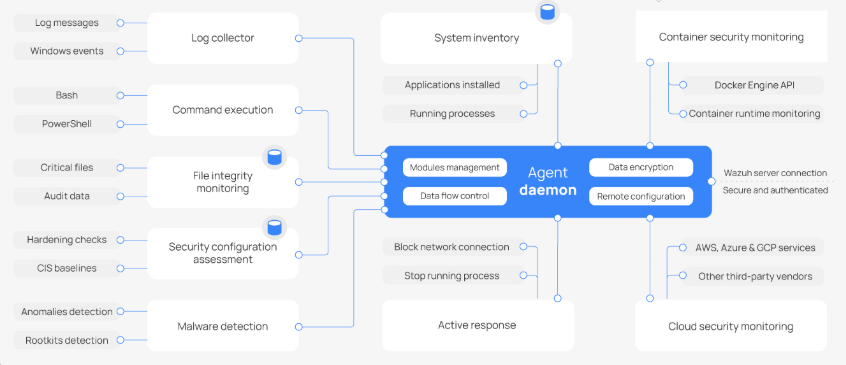
\includegraphics[width=0.9\textwidth]{figs/Wazuh_Agent_Architecture.png}}
\caption{Wazuh Agent Architecture}
\label{fig:Wazuh_Agent_Architecture}
\end{figure}

The Wazuh Server analyzes data received from agents and generates alerts when threats or suspicious patterns are detected. It also manages agent registration, validates agent identity, encrypts communication, distributes centralized configuration, and exposes a RESTful API for infrastructure management \cite{wazuh-server}. Its analysis engine is the component that transforms collected telemetry into security events usable by analysts and automation workflows.

\begin{figure}[H]
\centering
\fbox{
\includegraphics[width=0.9\textwidth]{figs/Wazuh_Server_Architecture.png}}
\caption{Wazuh Server Architecture}
\label{fig:Wazuh_Server_Architecture}
\end{figure}

The Wazuh Indexer provides scalable full-text search and analysis for Wazuh alerts and events. It stores data in JSON document format and supports near real-time querying. Wazuh uses several indices to separate alerts, archives, monitoring data, and statistics. The \texttt{wazuh-alerts} index stores events that trigger sufficiently important rules, \texttt{wazuh-archives} stores all received events, \texttt{wazuh-monitoring} stores agent status over time, and \texttt{wazuh-statistics} stores performance data \cite{wazuh-indexer}.

The Wazuh Dashboard provides the analyst interface used to explore, visualize, and manage security events. It supports event analysis, report creation, agent monitoring, platform management, log inspection, and rule testing \cite{wazuh-dashboard}. In the SOCaaS architecture, it complements the automated pipeline by giving analysts a direct view of endpoint status and alert evidence.

% ========== 3.6 SOAR CHOICE ==========
\section{SOAR Choice}
\label{sec:soar}

SOAR, or Security Orchestration, Automation and Response, is required to connect detection with structured response. While the SIEM identifies suspicious events, the SOAR layer coordinates enrichment, notification, case creation, and response actions. In this design, the SOAR family is considered through three complementary functions: security orchestration and automation, security incident response platform, and threat intelligence platform.

\subsection{SOA: Shuffle}
\label{subsec:shuffle}

Shuffle was selected as the security orchestration and automation component because it supports workflow-based automation and integration with external tools. It was designed to address challenges commonly encountered by CERT and SIRT teams, including ticket management, indicator handling, threat information processing, and integration with heterogeneous security services \cite{shuffle-docs}. In SOCaaS, Shuffle receives normalized alerts from the detection pipeline and executes the response workflow.

\subsubsection{Architecture}
\label{subsubsec:shuffle-arch}

Shuffle is organized around a server layer and worker execution units. The server hosts the core application functions, including API activity, workflow storage, validation, and scheduling. Workers operate as autonomous execution units that process actions defined in workflows. This separation supports scalability, because workers can be distributed across hosts or clustered depending on operational needs \cite{shuffle-arch}.

\textbf{Single server installation:}

\begin{figure}[H]
\centering
\fbox{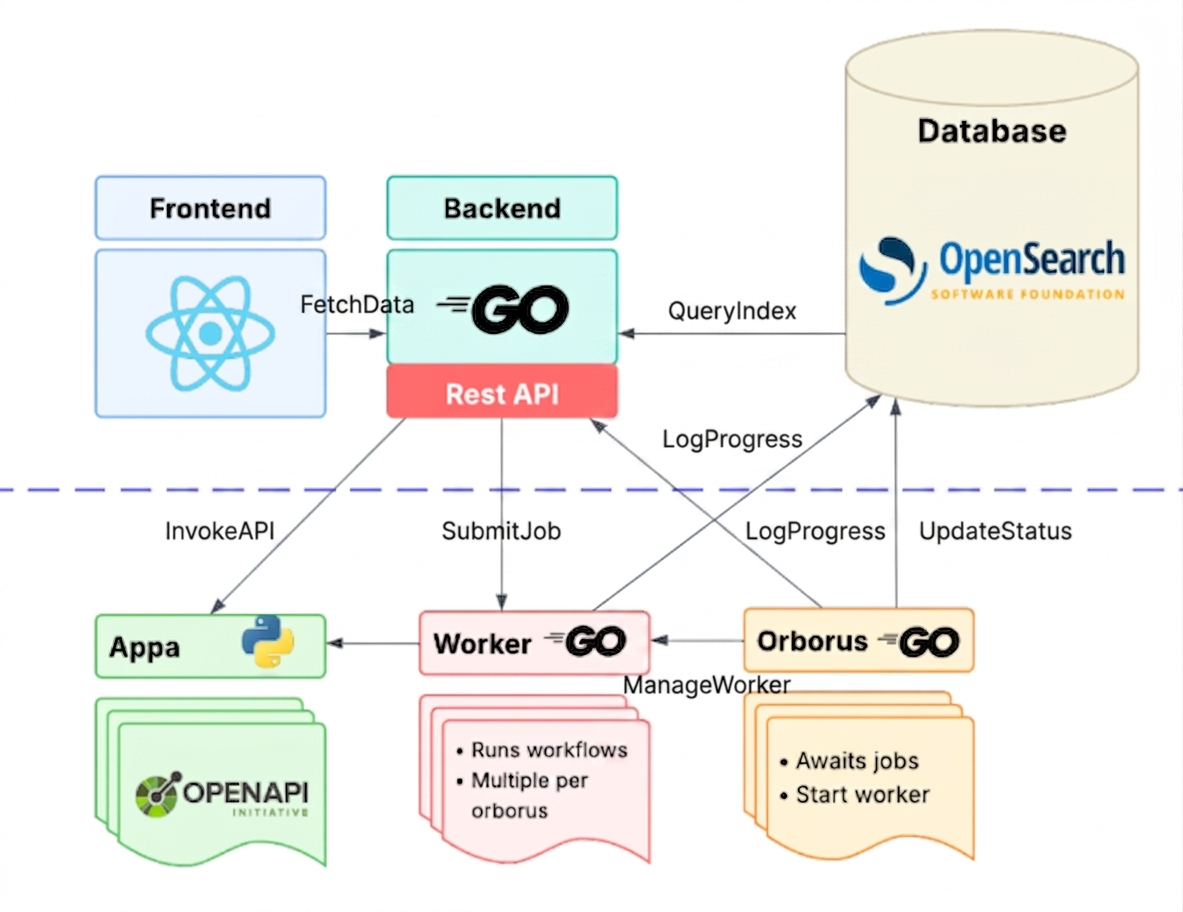
\includegraphics[width=0.9\textwidth]{figs/Shuffle_Architecture.png}}
\caption{Shuffle Architecture}
\label{fig:shuffle_architecture}
\end{figure}

\paragraph{1. Frontend (Graphical User Interface)}
\label{par:shuffle-frontend}

The Shuffle frontend is developed in ReactJS and provides the visual interface through which analysts and administrators create, manage, and observe workflows. It supports drag-and-drop workflow construction, real-time execution visualization, and management of users, organizations, and applications. The graphical representation relies on libraries such as Cytoscape, while interface components are supported by Material UI.

\paragraph{2. Backend (Main Server)}
\label{par:shuffle-backend}

The backend is developed in Go and constitutes the main server component of the platform. It manages secure REST APIs, validates and stores workflows, schedules executions, controls users and organizations, and communicates with Orborus and Workers. In the SOCaaS design, the backend is responsible for coordinating the automation logic that connects detection, enrichment, notification, and case management.

\subsubsection{Datastore (Database)}

Shuffle uses OpenSearch as its datastore. This database stores workflow definitions, application configurations, execution metadata, and user or organization information. Its role is to preserve the operational state of the SOAR platform and make workflow history available for review and troubleshooting.

\subsubsection{Orborus (Worker Scheduler)}

Orborus is the worker scheduler in Shuffle. It deploys and supervises workers, monitors their status, and distributes workflow execution tasks to appropriate execution units. This scheduling function is important for automation reliability because SOC workflows may include several parallel actions, external API calls, and conditional branches.

\subsubsection{Workers (Execution Units)}

Workers are autonomous execution units responsible for processing workflow actions such as API calls, data manipulation, notification construction, and integration requests. Their ability to operate in parallel supports horizontal scalability and makes it possible to isolate or distribute automation workloads.

\subsubsection{Applications (Apps)}

Applications, or Apps, are integration modules that allow Shuffle to interact with external tools and services. They can be developed in Python or configured through an \texttt{appspec.yaml} file. Each App groups actions representing specific operations, such as sending a message, creating a case in TheHive, or calling an external API. Before an App can be used in a workflow, it must be activated and, when necessary, configured with credentials or environment parameters.

\subsubsection{Workflows}

Workflows are directed graphs that represent automated security processes. They are composed of logically connected nodes and may include conditions, loops, variables, and custom API calls. Each workflow execution is called a run and can be monitored to review errors, results, and intermediate outputs. In SOCaaS, workflows are central because they transform a SIEM alert into a sequence of enrichment, notification, case creation, and response-support actions.

\subsubsection{Triggers}

Triggers define how a workflow starts. Shuffle supports HTTP triggers such as webhooks, scheduled triggers based on periodic execution, and application-based triggers generated by integrations. For SOCaaS, HTTP triggers are particularly important because they allow alerts from the detection pipeline to enter the automation workflow with structured parameters that are reused in subsequent steps.

% ========== 3.6.2 SIRP: TheHive ==========
\subsection{SIRP: TheHive}
\label{subsec:thehive}

TheHive was selected as the security incident response platform because SOCaaS requires a structured environment for case creation, evidence management, collaboration, and investigation tracking. It provides a centralized workspace where analysts can transform alerts into cases, manage tasks, attach evidence, record observables, and follow the incident response process.

TheHive supports collaboration between analysts through live updates on cases, tasks, observables, and indicators of compromise. It also supports integration with MISP, import of data from sources such as email reports, CTI providers, and SIEM alerts, and the use of templates to standardize case and task creation. These features make it suitable for SOCaaS because the platform must preserve investigation evidence while enabling automation through Shuffle \cite{thehive-docs}.

\subsubsection{Key Features}

The main value of TheHive lies in its ability to combine case management, collaboration, evidence handling, observable management, and threat intelligence enrichment. Analysts can record their investigation progress, attach files, add tags, import suspicious archives, and manage observables individually or in bulk. Analyzer and responder integrations can enrich investigations and accelerate containment decisions. This functionality complements the SOAR layer by providing a persistent incident record after automated triage has been performed.

\subsubsection{Architecture}

TheHive can be installed on a single server or deployed in a clustered architecture according to scalability requirements. Its modular design separates the main application, database, search index, and file storage. This separation allows the platform to scale and improves resilience when deployed in a production environment.

\paragraph{1. TheHive (Main Application)}

TheHive is the main application and provides the web interface used by analysts to create, track, and collaborate on cases. It also allows the analysis of observables and supports deployment either as a standalone instance or in a cluster, depending on availability and scalability needs.

\paragraph{2. Apache Cassandra (Database)}

Apache Cassandra is the distributed NoSQL database used by TheHive to store case information, tasks, observables, and related entities. Its architecture avoids a single point of failure and supports high availability. In a clustered configuration, at least three Cassandra nodes with a replication factor of 3 are recommended to provide data redundancy.

\begin{figure}[H]
\centering
\fbox{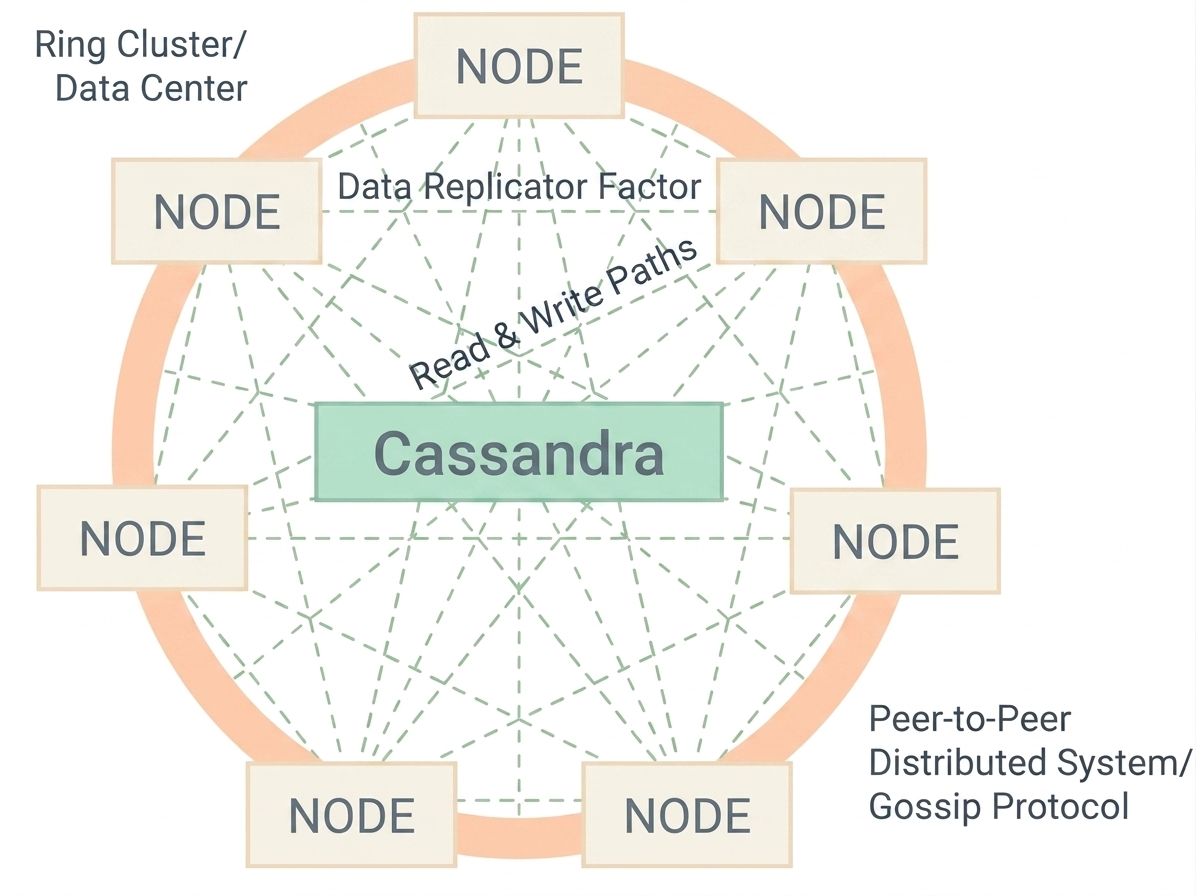
\includegraphics[width=0.8\textwidth]{figs/Cassandra.png}}
\caption{Apache Cassandra Architecture}
\label{fig:cassandra}
\end{figure}

\paragraph{3. Elasticsearch (Indexing Engine)}

Elasticsearch is used by TheHive to index and search case and observable data efficiently. Its role is to make incident records searchable and to support correlation during investigations. TheHive is compatible with Elasticsearch versions 7.x and 8.x, and OpenSearch can also be used as an alternative indexing engine.

\begin{figure}[H]
\centering
\fbox{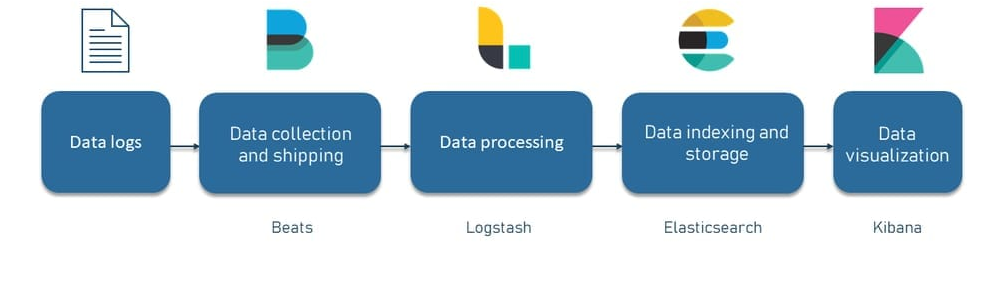
\includegraphics[width=0.8\textwidth]{figs/Elasticsearch.png}}
\caption{Elasticsearch Architecture}
\label{fig:elasticsearch}
\end{figure}

\paragraph{4. MinIO (Object Storage)}

MinIO is an S3-compatible object storage solution used by TheHive to store files associated with cases, including attachments, evidence, and reports. Its horizontal scalability and high availability are useful in clustered environments, where TheHive nodes may access shared storage through a load balancer.

\begin{figure}[H]
\centering
\fbox{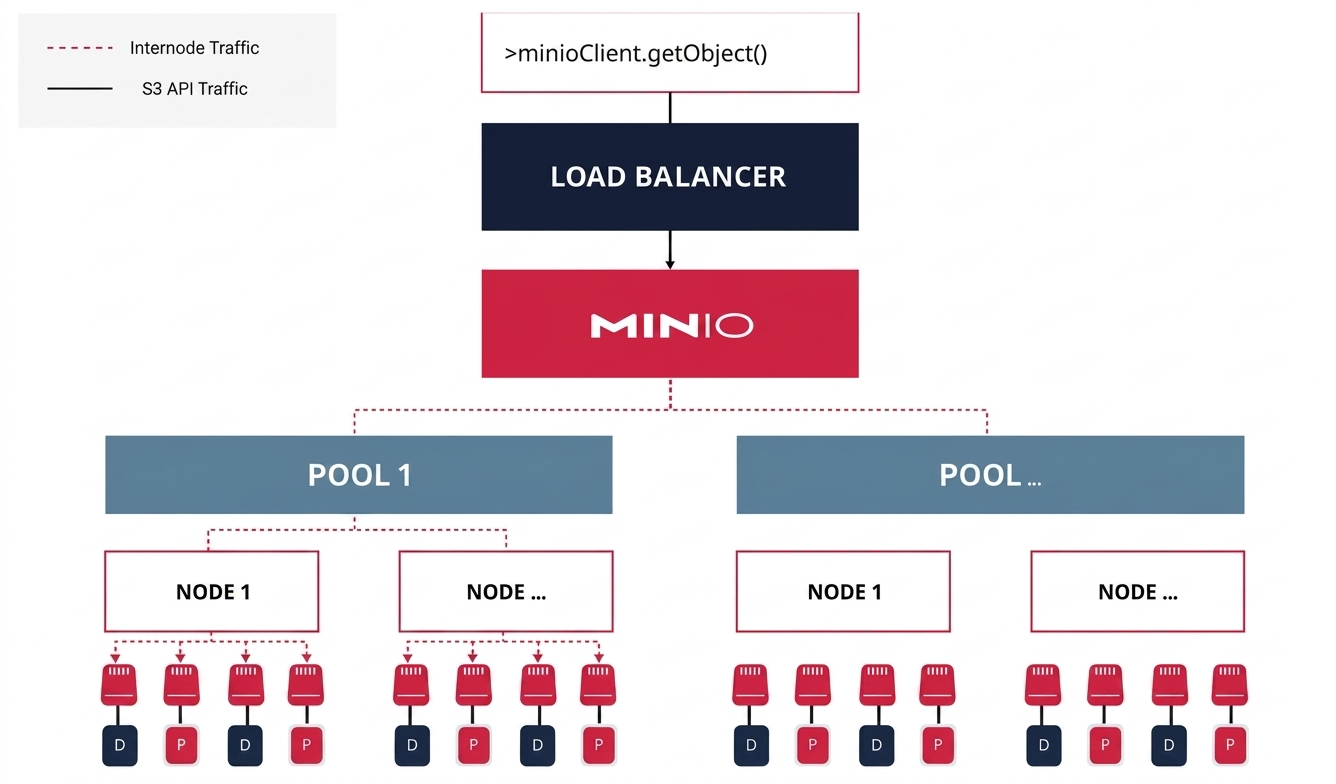
\includegraphics[width=0.8\textwidth]{figs/MinIO.png}}
\caption{MinIO Object Storage Architecture}
\label{fig:minio}
\end{figure}

% ========== 3.6.3 TIP ==========
\subsection{TIP: Threat Intelligence Platform}
\label{subsec:tip}

Threat intelligence enrichment is necessary in a SOAR architecture because raw observables rarely provide enough context for analyst decision-making. Public APIs such as VirusTotal, AbuseIPDB, and IPinfo can provide information about suspicious files, IP addresses, URLs, domains, and identities. In SOCaaS, these services are used to enrich alerts and improve the quality of automated triage.

\subsubsection{VirusTotal}

VirusTotal is a file and URL analysis service that relies on more than 70 antivirus engines, URL scanners, and domain blocklisting services. It can extract indicators from submitted content and can be accessed through a web interface, desktop applications, browser extensions, or an HTTP-based API. Its API makes it suitable for SOCaaS workflows because file hashes, URLs, or domains extracted from alerts can be checked automatically during triage.

\subsubsection{EmailRep}

EmailRep provides enrichment for email addresses, domain names, and digital identities. It relies on crawlers, scanners, and reputation data collected from sources such as social media profiles, professional networking sites, dark web credential leaks, data breaches, phishing kits, malicious emails, spam lists, open mail relays, and domain reputation indicators. In a SOCaaS context, this type of enrichment helps analysts evaluate whether an email-related observable is suspicious and whether it should influence incident priority.

% ========== 3.7 LOAD BALANCER ==========
\section{Load Balancer}
\label{sec:loadbalancer}

A load balancer distributes workload across multiple servers or services. In web and cloud environments, this mechanism reduces the load on individual servers, improves availability, and contributes to lower latency \cite{loadbalancer}. For SOCaaS, load balancing is relevant because several platform services require controlled external access, including dashboards, APIs, and automation endpoints.

\subsection{HAProxy}
\label{subsec:haproxy}

HAProxy is an open-source load balancer that supports TCP and HTTP/HTTPS traffic \cite{haproxy-docs}. It was selected because it can expose and distribute access to services while supporting health checks and access-control mechanisms. In the proposed architecture, HAProxy contributes to service availability and controlled external access for Kubernetes-hosted components.

\subsubsection{Characteristics of HAProxy}

HAProxy supports high-performance traffic distribution and is suitable for modern environments such as microservices and cloud deployments. It can use algorithms such as round robin, least connections, and source IP hash to distribute requests according to operational needs. It also performs health checks over HTTP or TCP to verify backend availability. From a security perspective, it can contribute to basic traffic filtering and rate control through access control lists and rate-limiting mechanisms.

\begin{figure}[H]
\centering
\fbox{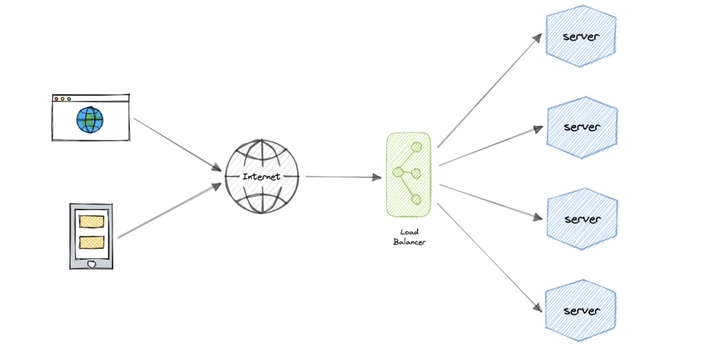
\includegraphics[width=0.8\textwidth]{figs/Load_Balancer.png}}
\caption{Load Balancer Architecture}
\label{fig:load_balancer}
\end{figure}

% ========== 3.8 SOC PLATFORM OPERATION ==========
\section{Operation of the SOC Platform}
\label{sec:operation}

The proposed SOC platform operates as a continuous detection and response pipeline. The process begins with data and log collection from endpoints, operating systems, network equipment, cloud applications, databases, and security tools. These logs are centralized through lightweight agents and standardized protocols in order to provide visibility across the monitored infrastructure.

Once collected, data is normalized, indexed, and stored in the Wazuh Indexer to support rapid search and analysis. Retention policies ranging from 30 to 90 days can be applied according to legal and operational requirements. This storage layer is essential because analysts must be able to reconstruct incident timelines and correlate new alerts with previous events.

The analysis phase relies on detection rules and queries that identify suspicious behavior, including patterns aligned with the MITRE ATT\&CK framework. Examples include lateral movement indicators, data exfiltration behavior, or repeated authentication failures followed by a successful login. When anomalies are detected, alerts are generated and classified according to severity. These alerts include contextual metadata such as source IP address, concerned user, endpoint information, and event type.

After alert generation, the triage process filters noise, prioritizes relevant events, and extracts observables such as IP addresses, file hashes, suspicious URLs, domains, and abnormal behaviors. These observables are enriched through threat intelligence sources to evaluate reputation and possible association with known malicious activity. Once the threat is characterized, appropriate playbooks are executed through the SOAR layer to support notification, case creation, enrichment, and response coordination.

This operational flow shows how the selected components interact as a single SOCaaS architecture. Wazuh provides detection and indexing, Shuffle provides orchestration and automation, TheHive preserves case evidence, threat intelligence platforms enrich observables, and HAProxy supports controlled access to exposed services.

\begin{figure}[H]
\centering
\fbox{\parbox{0.8\textwidth}{\centering\vspace{2cm}\textit{Figure 3.9 -- SOC Platform Operation}\vspace{2cm}}}
\caption{SOC Platform Operation}
\label{fig:soc-operation}
\end{figure}

% ========== 3.9 CONCLUSION ==========
\section{Conclusion}
\label{sec:ch3-conclusion}

This chapter presented the design logic of the SOCaaS platform and justified the selection of its principal components. The proposed architecture relies on Kubernetes and Helm to provide a reproducible cloud-native deployment foundation, Wazuh to perform endpoint monitoring and alert generation, Shuffle to automate triage and response workflows, TheHive to manage cases and investigation evidence, threat intelligence services to enrich observables, and HAProxy to support controlled access to exposed services.

The selected technologies form a coherent SOCaaS architecture because each component addresses a distinct operational requirement while remaining interoperable with the others. Kubernetes and Helm make the deployment reusable, Wazuh provides detection visibility, Shuffle connects alerts to automated actions, TheHive gives analysts a structured investigation workspace, and enrichment services improve alert context. Supporting elements such as KVM/QEMU, DeepSeek-V4-Pro, and OpenCode complement this design respectively at the laboratory infrastructure, AI-assisted reporting, and engineering workflow levels. This design therefore establishes the technical basis required for the implementation and validation phase presented in Chapter~4.

\begin{comment}
% ========== BIBLIOGRAPHY ==========
\begin{thebibliography}{99}
\bibitem{k8s-docs} Kubernetes Documentation, \textit{Kubernetes Components}, available at: \url{https://kubernetes.io/docs/concepts/overview/components/}
\bibitem{helm-docs} Helm Documentation, \textit{Helm -- The package manager for Kubernetes}, available at: \url{https://helm.sh/docs/}
\bibitem{wazuh-community} Wazuh, \textit{Wazuh Community}, available at: \url{https://wazuh.com/community/}
\bibitem{wazuh-agent} Wazuh Documentation, \textit{Wazuh Agent}, available at: \url{https://documentation.wazuh.com/current/installation-guide/wazuh-agent/index.html}
\bibitem{wazuh-server} Wazuh Documentation, \textit{Wazuh Server}, available at: \url{https://documentation.wazuh.com/current/installation-guide/wazuh-server/index.html}
\bibitem{wazuh-indexer} Wazuh Documentation, \textit{Wazuh Indexer}, available at: \url{https://documentation.wazuh.com/current/installation-guide/wazuh-indexer/index.html}
\bibitem{wazuh-dashboard} Wazuh Documentation, \textit{Wazuh Dashboard}, available at: \url{https://documentation.wazuh.com/current/installation-guide/wazuh-dashboard/index.html}
\bibitem{shuffle-docs} Shuffle, \textit{Shuffle Documentation}, available at: \url{https://shuffler.io/docs/about}
\bibitem{shuffle-arch} Shuffle, \textit{Shuffle Architecture}, available at: \url{https://shuffler.io/docs/architecture}
\bibitem{thehive-docs} TheHive Documentation, \textit{TheHive - Security Incident Response Platform}, available at: \url{https://docs.thehive-project.org/}
\bibitem{loadbalancer} Load Balancer Definition, available at: \url{https://en.wikipedia.org/wiki/Load_balancing_(computing)}
\bibitem{haproxy-docs} HAProxy Documentation, \textit{HAProxy - The Reliable, High Performance TCP/HTTP Load Balancer}, available at: \url{https://www.haproxy.org/}
\end{thebibliography}
\end{comment}
